\chapter{Results}

%\section{Comparing the CNN to the currently used Random Forest}
After the optimizing process a \num{20} CNNs were trained with the gained insights.
A \enquote{\texttt{6c\_4f}} architecture was trained with the mentioned dropout rates
and \num{5000} batches of pretraining for every layer.
The hyperparameters were set by a random grid search.

For reviewing the best, trained network, a so far unused simulated dataset has been used.
As a result, the separation of hadrons and gamma rays through the CNN's processing can be observed and evaluated.
By processing \num{500000} events of both classes and plotting the resulting predictions,
a separation of those classes can be observed.
Although many events overlap and are therefore not separable,
both curves are slightly skewed to their respective end of the axes.
With this dataset, a ROC-AUC score of \num{0.817} can be achieved.

\begin{figure}
    \centering
    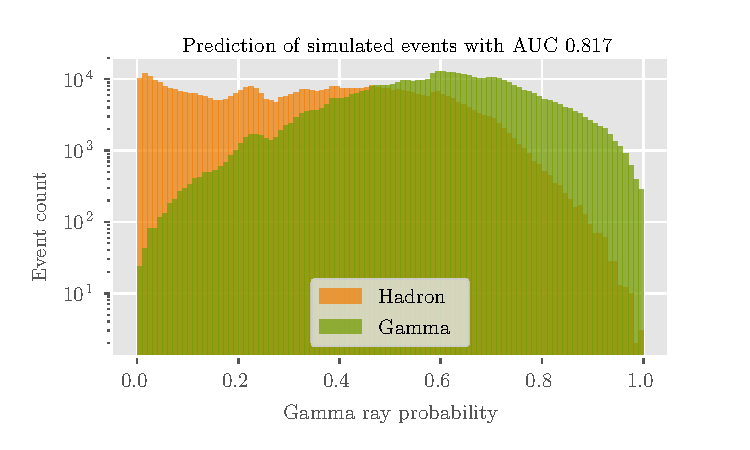
\includegraphics[scale=1]{Plots/CNN_MC_Evaluation.pdf}
    \caption{Using an unseen, simulated dataset for the evaluation of the CNN's performance, a separation of the two classes is visible.}
    \label{fig:cnn_mc_evaluation}
\end{figure}

In the best case a real-image dataset displays a similar distribution of the classes,
only distinguished from the simulated events by the ratio of hadrons to gamma rays.
The real-image dataset consists of data,
which has been recorded between \num{2013} and \num{2014} and shows the activity of the Crab nebula.
It contains roughly \num{20000000} events.

By comparing the histograms of the simulated and real datasets,
a distinctly smaller occurrence of gamma rays can be noted.
This could arise from a small ratio in the cosmic radiation
or a poor performance of the CNN caused by a mismatch between the real and simulated datasets.

\begin{figure}
    \centering
    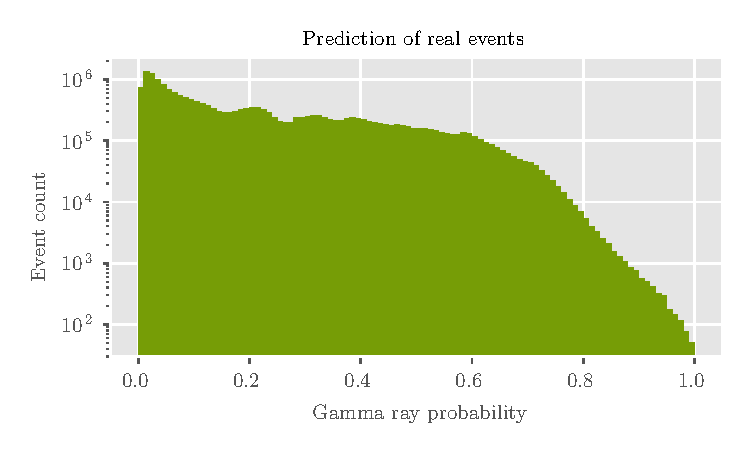
\includegraphics[scale=1]{Plots/CNN_Real_Evaluation.pdf}
    \caption{Using a real dataset of the Crab nebula, the predictions imply a high rate of hadrons and a small rate of gamma rays in the cosmic radiation.}
    \label{fig:cnn_real_evaluation}
\end{figure}

Since the Crab nebula is a well surveyed source by many telescopes around the globe,
it should be detectable with the newly predicted gamma rays at its position.
Since every gamma ray can be retraced to its origin,
the gamma ray activity of six opposing positions in FACT's field of view will be compared.
The first position (\enquote{On}) is the calculated position of the Crab nebula
and contains activities of the source and the background radiation.
The five other positions (\enquote{Off}) lie circular and equally spaced next to the first one
and therefore contain only background radiation.
In this way a difference of activity at the Crab nebula position can be detected.

The positions will be compared using a Theta-plot.
Both position's centers are placed at zero on the x-axis.
The x-axis measures the angular distance to this position,
while the y-axis depicts the activity of the cosmic region.
The crucial significance value summarizes this difference.
In this case, the Crab nebula can be detected with \num{24.4}\,$\sigma$.
Since comparable approaches with currently used Random Forest classifiers reach \num{39.89}\,$\sigma$ \cite{significance},
a poor performance of the CNN can be assumed.

\begin{figure}
    \centering
    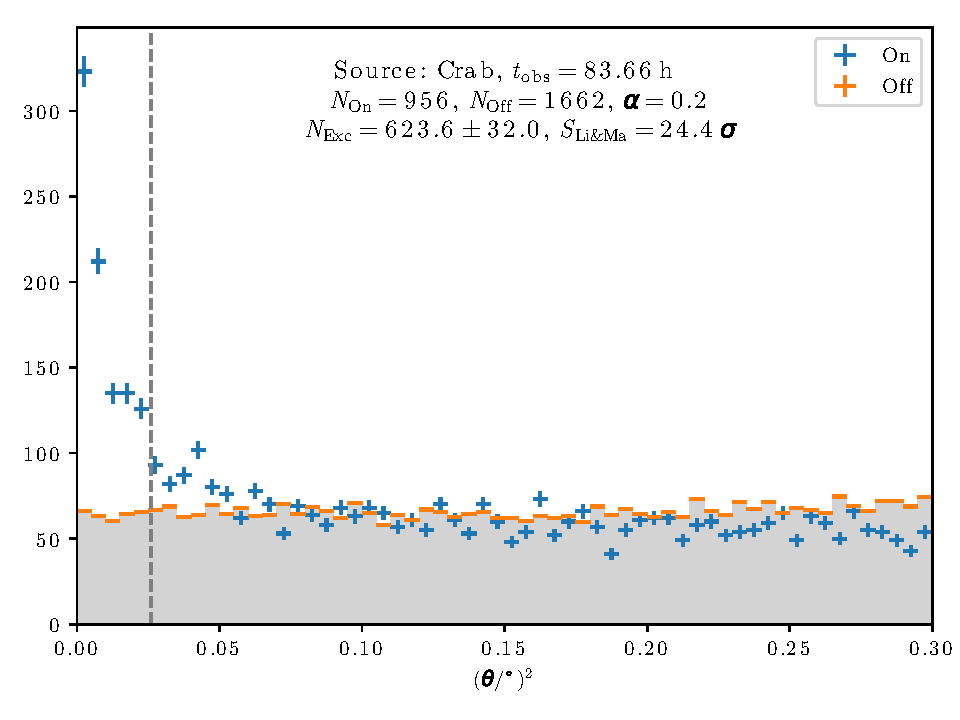
\includegraphics[scale=0.8]{Plots/Theta_Plot.pdf}
    \caption{After \num{83.7}\,\si{\hour} of observation time the Crab nebula can be seen with the CNN with a significance of \num{24.4}\,$\sigma$.}
    \label{fig:theta_plot}
\end{figure}

This poor performance can derive from two distinct origins:
either the network can be optimized to overcome the performance difference
or the simulated input data contains features which the CNN utilizes,
that are absent in the real images (Monte Carlo Mismatch).
Since much effort has been put into optimizing the network,
only small prospective improvements can be expected from further optimization.
Therefore, the big performance difference seems to emerge from a mismatch between the training dataset and the real images.


\chapter{Conclusion}
\section{Potential Enhancements}
To enhance the network's performance, there are two different approaches:
on the one hand, there is the possibility of changing the input data;
on the other hand, there are further options to improve the network's structure and data handling.
Options to improve results will be described in the following paragraph.
The order follows the data's pathway through the network and its programs.

First and foremost a simulated dataset has been used and the downside of this has been described.
The mismatch between simulated and real data seems to arise a malfunction when predicting real images.
Improving this dataset would be a complex and time-consuming task without any improvement guarantees.
As this may not solve the problem,
a more promising approach could be to switch from generated images to real images.
The current classifier could predict labels for each real image, and these labels
and images would form the training data for the network.
In contrast to the first approach, uncertain labels would be the main challenge to overcome.

Additionally, the flat hexagonal structure has been skewed to fit into a flat square structure.
Alternatively, a two-dimensional hexagonal structure could be transformed to a three-dimensional cubic structure
without losing any neighborhood information at all.
Furthermore, the time series information has been lost in this thesis by summing it up.
In contrast to a two dimensional convolution with loss of information, as performed in this thesis,
a four dimensional convolution with all information could be performed for the feature generation.
For this, the library \texttt{TensorFlow} will not be sufficient as such high dimensional convolutions are not yet supported.

Although many architectures have been implemented and many hyperparameters have been evaluated,
only a small feature space could be investigated in this thesis.
Naturally, expanding the hyperparameter optimization could yield better results.
Since all hyperparameters form a feature space themselves, a machine learning algorithm could be designed to predict
a network's performance by using the hyperparameters as input.
To optimize a network's performance during the training,
a reinforcement learning algorithm (Q-Learning) could increase the network's performance.
Rewarding the reinforcement learner for increasing the best performance,
could achieve a more optimized network overall \cite{q_learning}.

As the mismatch in the data will not be overcome by increasing the performance of the network itself,
the training data must first of all be exchanged.
After that, the network proposed in this thesis could investigate the performance using the new data
instead to the simulated data used here.
Once this has been successful, the other suggestions could be implemented.


\section{Outlook}
To classify images originating from cosmic radiation, a Convolutional Neural Network has been trained on a simulated dataset.
This network has been optimized, evaluated and performs comparably to the currently-used Random Forest on this task.
By predicting real images and computing the significance of the Crab nebula, a crucial performance difference between
the CNN and the other classifiers emerges.
Since CNNs have outperformed other classifiers in image classification tasks in the past,
this gap cannot be explained by a poorly optimized network alone.
The known mismatch in the simulated training dataset and the real images can be again confirmed.
To overcome this problem, an improved training dataset is the most promising option.
As simulated datasets contain the threat of mismatches every time,
training the CNN on real images could be the solution.
This introduces the challenge of creating a dataset containing real images with reliable labels.
As a first step, the current classifiers could be used to label the images.
The most reliable images could serve as the training data for a CNN.
This CNN's performance could yield new insights as to whether this approach is encouraging.
